\documentclass[twocolumn]{article}

\usepackage{biblatex}
\usepackage{graphicx}
\usepackage[plain]{fancyref}

\addbibresource{breastMassDetection.bib}

\title{A Deep Learning Approach for Breast Cancer Mass Detection : A Review}

\author{
  Omar Emara (20180364), Omar Khaled (20180367) \\
  Ibrahim Magdy (20180014), Ahmed Nasser (20160052), Moataz Nasr (20180614)
}

\begin{document}

\maketitle

\begin{abstract}

  Breast cancer is one of the fastest growing types of cancer and is one of the
  leading cause of cancer death for women around the globe. Consequently, early
  detection is of essence in death prevention. Detection is typically done by
  \emph{Mammography Screening}, either manually by doctors or with the help of
  recently developed computer aided automatic screening systems, which helps
  make better and more accurate predictions. Advances in machine learning and
  the greater availability of public mammography datasets allowed researches to
  develop machine learning models that achieve even greater accuracy. In this
  article, we shall review once such research paper \autocite{Fathy2019}, titled
  "A Deep Learning Approach for Breast Cancer Mass Detection". Additionally, a
  Tensorflow implementation is presented.

\end{abstract}

\section{Introduction}

The paper \autocite{Fathy2019}, which we shall review, describe a \emph{Transfer
Learning} approach to detect the existence of breast masses in mammogram images
and localize those masses if they exist. The paper proposes a model based on a
pre-trained ResNet-50 model similar to the one described in \autocite{He2016}.
Moreover, the paper utilizes the algorithm described in \autocite{Zhou2016} to
construct a \emph{Class Activation Map (CAM)} which serve to localize the breast
masses if they exist. Each of those are presented in one of the following
sections.

\section{Dataset}

The paper utilizes a subset of the \emph{Digital Database for Screening
Mammography (DDSM)} published in \autocite{Bowyer1996} and \autocite{Heath1998}.
The paper selected 2517 mammograms for training, 629 for validation, and 786 for
testing.

Unfortunately, the size of the dataset was too large for us to download and
utilize, even if we consider a subset. Consequently, we considered other curated
versions of the dataset, mainly the CBIS-DDSM dataset presented in
\autocite{Lee2017}. But even this dataset was very large for us to use. So we
used a smaller version published in \autocite{Luka2020}. This dataset is cropped
and re-sampled around the \emph{Region Of Interest (ROI)} available in the
meta-data of the original dataset. The mammograms have a resolution of $900
\times 900$.

\section{Preprocessing}

The paper describe a number of preprocessing procedures to be performed on the
mammograms. First, the breast region is masked and tightly cropped around the
mask. The mask is generated using the \emph{ST Segmentation} technique described
in \autocite{Pertuz2014}. We didn't need to perform this step because the
dataset we use already cropped the mammograms around the ROI.

Next, the mammograms are processed to be suitable for the ResNet-50 model. The
model requires the images to be of resolution $224 \times 224$, to have three
color channels of format \texttt{BGR}, and to have zero centered values relative
to the ImageNet dataset. The latter requirement can be achieved using the
\texttt{preprocess\_input} function of the \texttt{resnet} module of Tensorflow.

\section{Model}

The paper built the model based on the ResNet-50 pre-trained model. The model is
created without the last prediction layer, then a dense layer with a single unit
and a sigmoid activation function is appended to the model, where it is
connected to the last \emph{Global Average Pooling} layer. The model is compiled
using the Adam optimizer with a binary cross entropy loss function with a batch
size of 16 and a learning rate of 0.001.

While the paper fine-tune the whole network, this was unfeasible for us due to
the computational intensive nature of the training. Consequently, we froze the
weights of the model except for the last prediction dense layer. The training
was done using an early stopping condition with a patience level of 5 and the
best model with respect to the binary accuracy of the validation dataset was
saved. The training stopped after 9 epochs due to the early stopping condition.

\section{Class Activation Map}

While the model can classify the mammogram and predict if a breast mass exist,
it doesn't predict where the mass is, or at least what part of the mammogram
promoted that prediction. The CAM method was proposed to allow such
localizations to be done. In the ResNet-50 architecture, the last convolution
layer, named \texttt{conv5\_block3\_out}, is composed of 2048 activation maps of
dimensions $7 \times 7$. Each of those maps is reduced to a single value in the
following global average pooling layer producing the feature vector that is
eventually used for fitting the last dense layer. If each of the 2048 activation
maps are weighted by their corresponding last-layer-weights and summed, the
result will be the activation map that promoted the prediction, which
essentially gives a hint on localizing the mass, albeit a low resolution one. In
the case of binary classification, the class activation map is given by:

\begin{equation}
  C(x, y) = \sum_{i = 1}^{2048}{W_i F_i(x, y)}
\end{equation}

Where $C(x, y)$ is the desired class activation map value at the position $(x,
y)$, $F_i(x, y)$ is the value of the $i$th activation map in the last
convolution layer at the position $(x, y)$, and $W_i$ is the weight of the
corresponding connection to the last dense layer. \Fref{fig:ClassActivationMap}
shows one such class activation map.

\begin{figure}
\begin{center}
  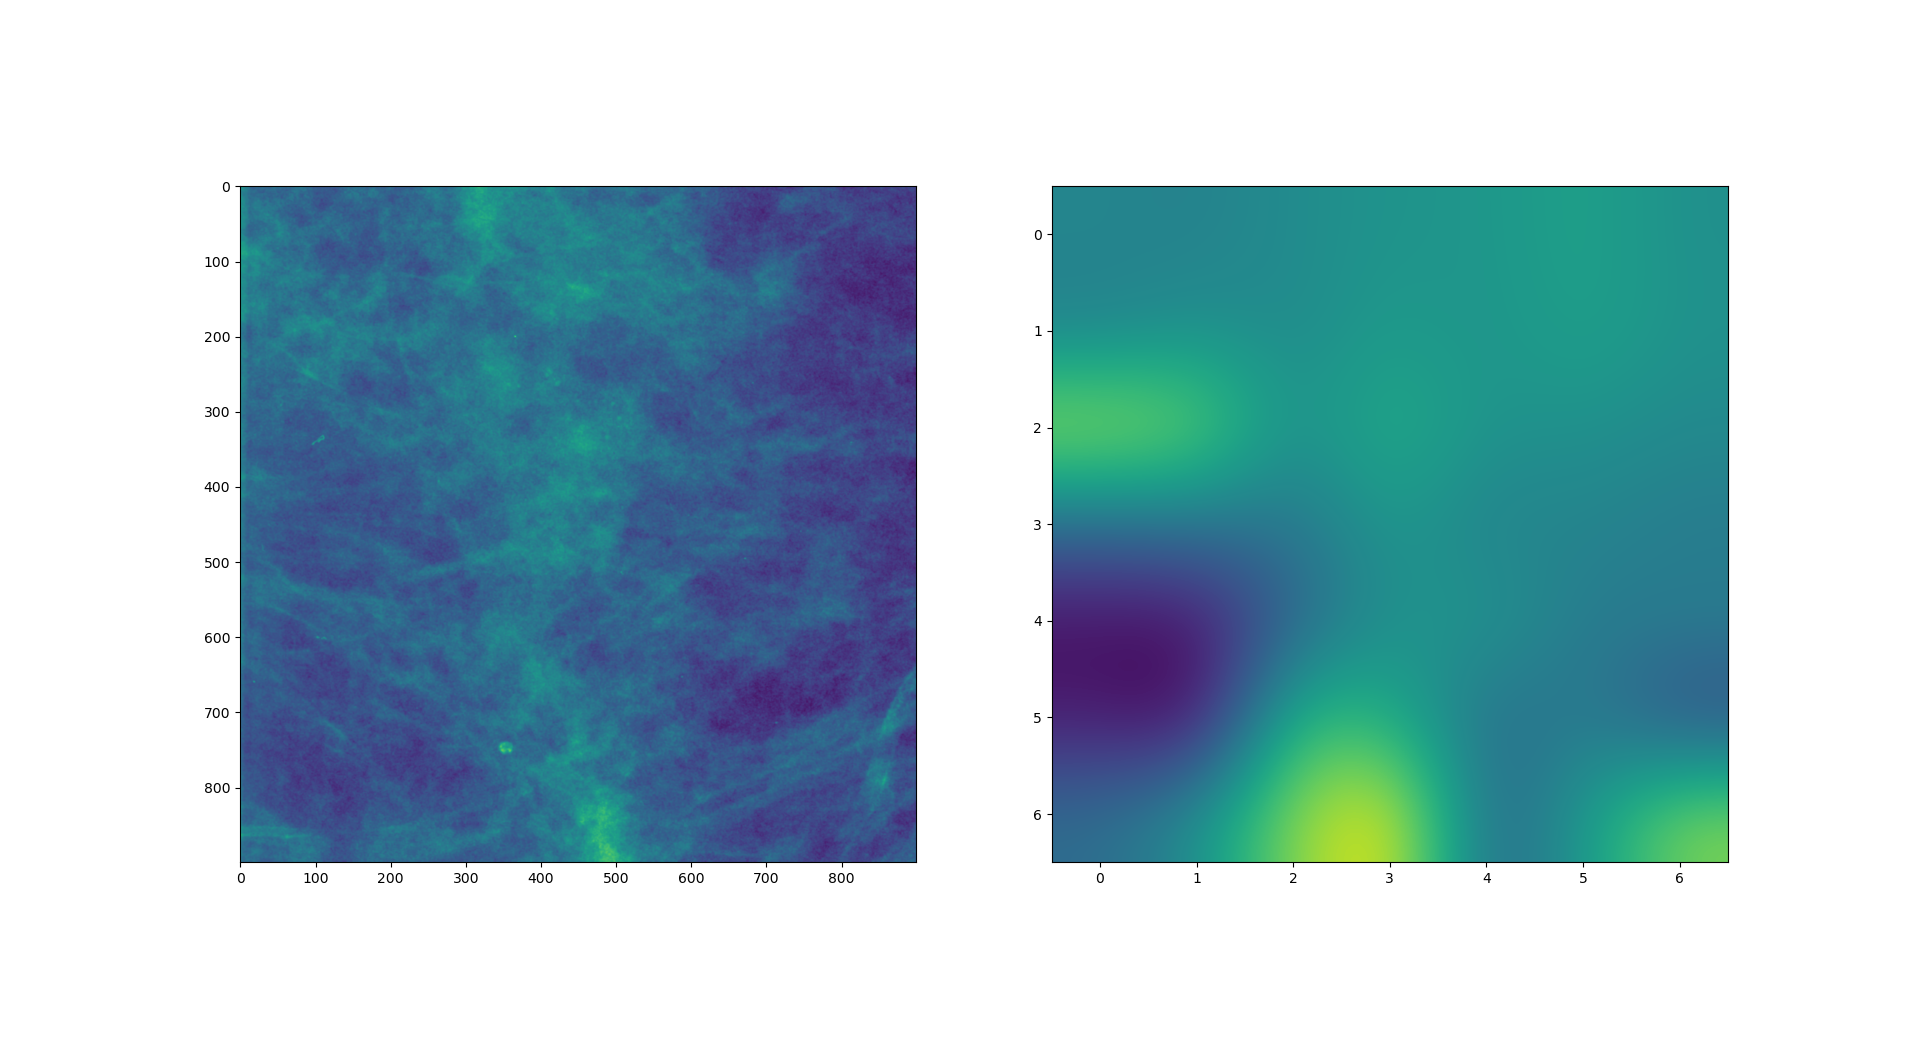
\includegraphics[width=0.5\textwidth]{classActivationMap}
\end{center}
\caption{An example class activation map for a mammogram with a mass. Bright
  areas denote higher significance.}
\label{fig:ClassActivationMap}
\end{figure}

\section{Conclusion}

Our implantation of the paper achieved a binary accuracy of 77\% on the testing
dataset. This is a much lower accuracy compared to the results of the paper,
this is likely due to the corners we cut when it comes to fine tuning the model
and the use of a smaller dataset.

\printbibliography

\end{document}
